\chapter{Kravspecifikation}

%Moscow
Produktets krav er prioriteret ved brug af MoSCoW metoden. Her er kravene inddelt i fire overordnede kategorier, hvor de vigtigste elementer er prioriteret højest. \textbf{Must} benævner de krav som skal opfyldes, og som er essentielle for produktets funktionalitet. \textbf{Should} er de krav produktet bør opfylde, men udvikling af disse bør først begyndes når vigtigere krav er opfyldt. \textbf{Could} er krav som produktet evt. skal opfylde, hvis projektets tidsramme tillader det. Dette er ofte ekstra features, eller optimering af brugervenlighed. \textbf{Won't} er krav som ikke vil blive opfyldt, men evt. kan tages med i en videreudvikling af produktet.

\noindent Følgende liste viser kravene for projektet:
\begin{itemize}
	\item[\textbf{Must}]
		\begin{itemize}
			\item Have et funktionsdygtigt power-modul
			\item Ikke påvirke andre moduler ved fejl
			\item Have stabil regulering
			\item Underbygges med en P-Spice model

		\end{itemize}
	\item[\textbf{Should}]
		\begin{itemize}
			\item Have programmerbar udgangsstrøm og -spænding
			\item Have et termisk design, kompatibelt med vakuum
			\item Have overstrømsbeskyttelse på udgangen
			\item Have overspændingsbeskyttelse på udgangen

		\end{itemize}
	\item[\textbf{Could}] 
		\begin{itemize}
			\item Have mulighed for brug til mere end to forskellige typer loads
			\item Konstrueres med EEE komponenter

		\end{itemize}
	\item[\textbf{Won't}]
		\begin{itemize}
			\item Have feedback til brugeren når valgt load er aktiveret
			\item Have galvanisk adskillelse
			
		\end{itemize}
\end{itemize}

\clearpage


\section{Load beskrivelse} \label{load_types}
I det følgende afsnit beskrives systemets to loads. Hver beskrivelse indeholder en kort beskrivelse af aktørens funktionalitet.


\begin{framed}
	\subsection{Thermal Knife load}

	\subsubsection*{Beskrivelse:}
	Thermal Knife load er en load type, hvor et varmelegeme opvarmes langsomt. \indent Denne type bruges til at skære reb over, og derved udløse diverse bevægelige \indent dele.
\end{framed}

\begin{framed}
	\subsection{Pyro load}
	
	\subsubsection*{Beskrivelse:}
	Pyro load er en load type, hvor en glødetråd opvarmes hurtigt. Denne type bru- \indent ges til at detonere en krudtladning, og derved sprænge en bolt af, som frigør \indent diverse bevægelige dele.
\end{framed}

\clearpage

\section{Flow diagram}
I dette afsnit beskrives flowet i systemet vha. et flow diagram. Det opstilles for at give et overblik over systemets flow, og hvilke scenarier der kan påvirke det. 

Starten initieres ved der vælges load type. Som udgangspunkt vælges der mellem Pyro load og Thermal Knife load, som begge er beskrevet i afsnit~\ref{load_types}. Her kan der tilføjes flere loads, hvis systemet ønskes tilpasset til flere typer. Hvis der ikke vælges en load type, skal systemet, som default, indstilles til Thermal Knife load. Nu bliver systemet initieret, ved at aktivere loaden. Dette starter de to reguleringssløjfer - spændingsreguleringen og strømreguleringen. Begge sløjfer tilpasser PWM-signalets duty-cycle, hvis det faktiske output ikke er lig det ønskede. Til sidst kontrolleres det om loaden skal deaktiveres, eller reguleringen skal fortsætte.

\begin{figure}[H]
	\center
	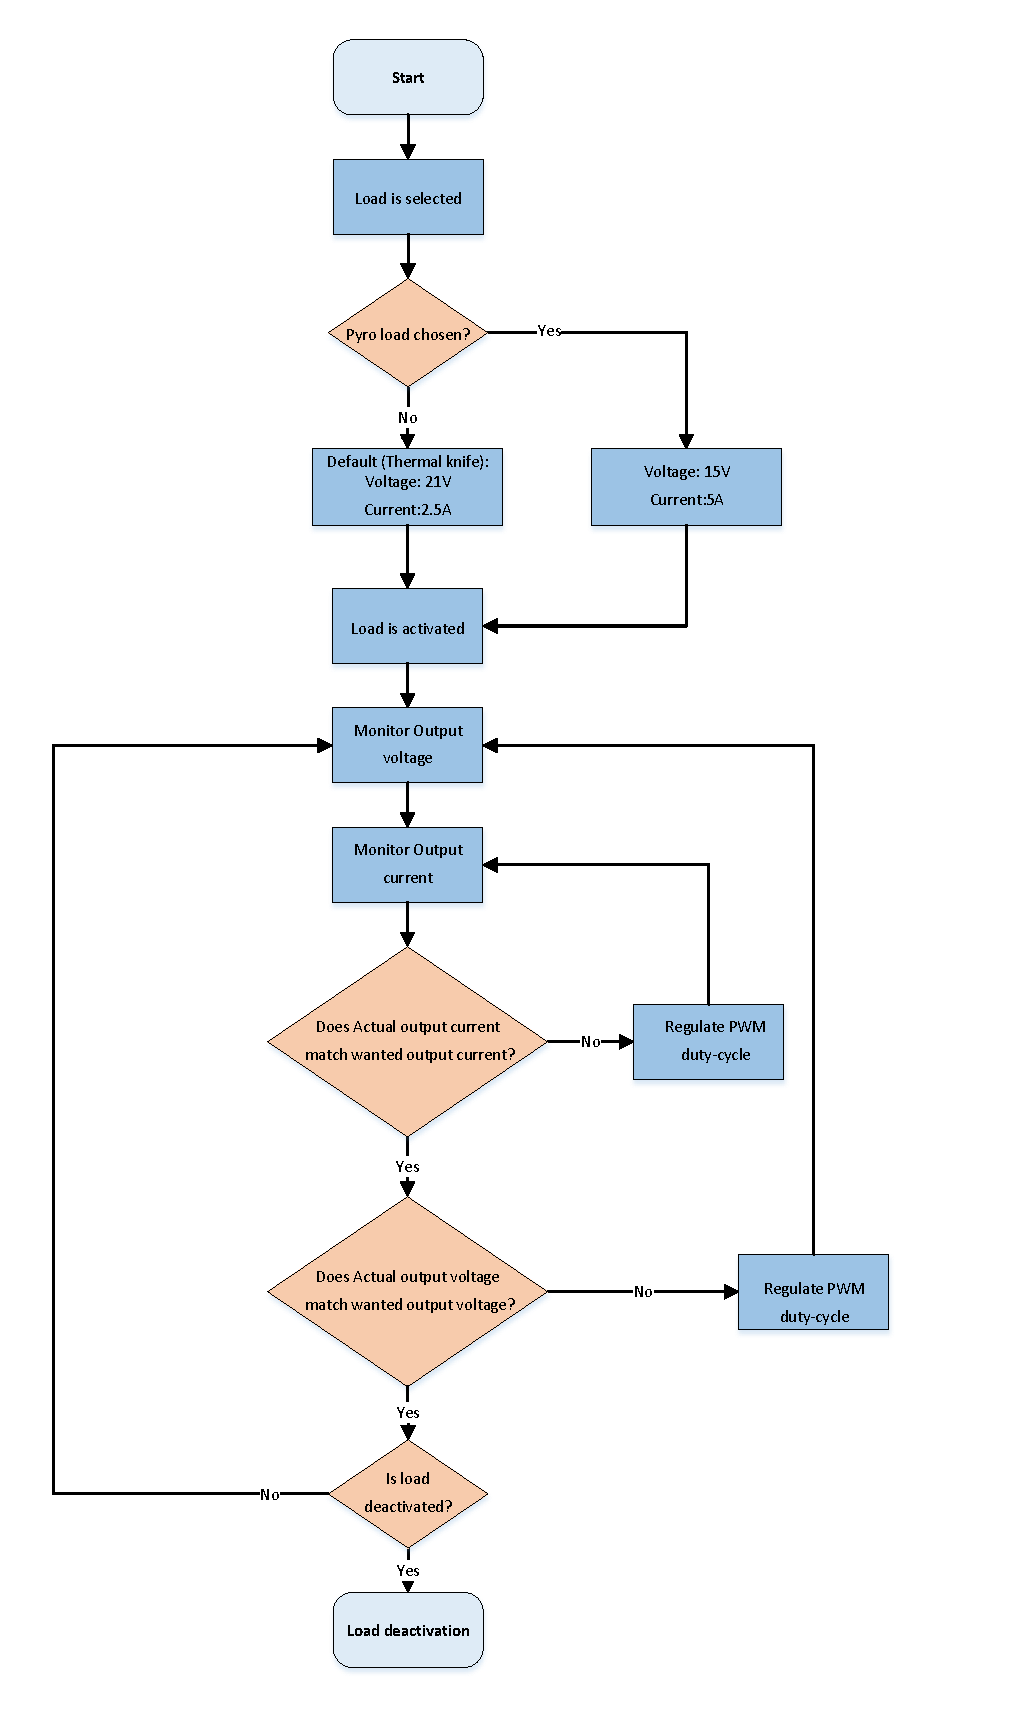
\includegraphics[max width=0.7\linewidth]{/tex/kravspecifikation/billeder/Flow_diagram.pdf}
	\caption{Flow diagram over systemet}
	\label{fig:flow_diagram}
\end{figure}

\clearpage

\section{Ikke-funktionelle krav}
I dette afsnit beskrives produktets ikke-funktionelle krav. Her opstilles f.eks. krav om præcision, effektivitet samt produktets dimensioner.
\begin{itemize}
			\item Converterens inputspænding skal være mellem 26-50V
			\item Converteren må maksimalt trække en peak-strøm fra inputkilden på 150\% af DC inputstrømmen
			\item Converteren skal opretholde en outputspænding på 21V, $\pm$2\% ved 2,5A $\pm$5\%
			\item Converteren skal opretholde en outputstrøm på 5A $\pm$5\%, ved 15V $\pm$2\%
			\item Converteren må maksimalt have en output ripple-spænding på 50mV pk-pk
			\item Converteren må maksimalt have switching spikes på 100mV pk-pk
			\item Converteren skal kunne omsætte op til 75W
			\item Converteren skal operere med et tab på maksimalt 5W %TODO Specificer tab nærmere
			\item Converteren skal implementeres i et volumen mindre end 17x75x100mm på forsiden af PCB'et, samt 3x75x100mm på bagsiden af PCB'et
			\item Converteren skal kunne operere med en omgivelsestemperatur mellem -35\degreeCelsius\  og 65\degreeCelsius\
			\item Converteren skal have stabil regulering med minimum 10dB gain margin og 50 graders fasemargin ved:
				\begin{description}
					\item 21V/2,5A ved 26V og 50V inputspænding
					\item 5A/3\ohm\ ved 26V og 50V indgangsspænding
				\end{description}
			\item Reguleringen skal have en risetime på maksimalt 0,5ms
			\item Reguleringen skal have et overshoot på maksimalt 5\% %TODO Specificer overshoot nærmere
					
\end{itemize}
